\documentclass[10pt,a4paper]{article}
\usepackage[utf8]{inputenc}
\usepackage{amsmath}
\usepackage{amsfonts}
\usepackage{amssymb}
\usepackage{graphicx}
\usepackage{hyperref}
\usepackage{caption}
\usepackage{subcaption}

\usepackage{listings}
\usepackage{color}

\definecolor{dkgreen}{rgb}{0,0.6,0}
\definecolor{gray}{rgb}{0.5,0.5,0.5}
\definecolor{mauve}{rgb}{0.58,0,0.82}

\lstset{frame=tb,
  language=Python,
  aboveskip=3mm,
  belowskip=3mm,
  showstringspaces=false,
  columns=flexible,
  basicstyle={\small\ttfamily},
  numbers=none,
  numberstyle=\tiny\color{gray},
  keywordstyle=\color{blue},
  commentstyle=\color{dkgreen},
  stringstyle=\color{mauve},
  breaklines=true,
  breakatwhitespace=true,
  tabsize=3
}


\begin{document}

%Proposal follows a well-organized structure and would be readily understood by its intended audience. Each section is written in a clear, concise and specific manner. Few grammatical and spelling mistakes are present. All resources used and referenced are properly cited.

\begin{titlepage}
	\centering
	\vspace{1cm}
	{\scshape\Large Udacity 2018: Capstone Project \par}
	\vspace{1.5cm}
	{\huge\bfseries Machine learning methods for Forecasting time series \par}
	\vspace{1.5cm}
	{\large\bfseries with applications to currency exchange rates \par}
	\vspace{2cm}
	{\Large Author: Oscar Javier Hernandez\par}
	\vfill

% Bottom of the page
	{\large \today\par}
\end{titlepage}

\section{Definition}
%(approx. 1-2 pages)
\subsection{Project Overview}\label{sec: overview}
%In this section, look to provide a high-level overview of the project in layman’s terms. Questions to ask yourself when writing this section:
%
%Has an overview of the project been provided, such as the problem domain, project origin, and related datasets or input data?
%Has enough background information been given so that an uninformed reader would understand the problem domain and following problem statement?
A set of data that is indexed by time is known as a time series. They appear in many different fields, such as statistics, physics, finance, economics, biology, or even business \cite{Adhikari_2013}. Because of their wide applicability, it is important to generate accurate forecasts of time series data. These forecasts are generated using specific mathematical models or algorithms which are trained on a subset of the past values of a given time series. For the purpose of simplifying future discussions, we will adopt the following notation for a time series, denoted $X_t$, as
\begin{equation}
\lbrace X_t; t=0,1,... \rbrace.
\end{equation}
Where $t$ denotes the time-index of the series. One of the simplest models for a time series is the ARIMA (Auto regressive integrated moving average) model. This model is denoted as ARIMA$(p,d,q)$ assumes that the time series $X_t$ has the form
\begin{equation}
X_{t} = \mu +\epsilon_t+ \sum_{i=1}^p \phi_i L^i \left[ (1-L)^d \right] X_{t} + \sum_{j=1}^q \theta_j \epsilon_{t-j},
\end{equation}  
where $\lbrace \phi_i | i=1,...,p \rbrace$, $\lbrace \theta_i | i=1,...,q \rbrace$ are model parameters and $L$ is the lag operator defined as $L X_t = X_{t-1} $. The parameter $p$, is known as the auto-regressive (${\rm AR}$) order, $d$ is the differencing order, and $q$ is the moving average parameter (MA). 

The term $\epsilon_{t}$ denotes the error terms, assumed to be independent, identically distributed random variables sampled from a zero-mean, normal distribution. The value $\mu$ denotes the average of this model. ARIMA models can be applied to make forecasts of stationary time series ( defined as a time series whose mean, variance and auto correlation does not change over time), or to a time series that can be transformed into a stationary time series. However, there are other state-of-the-art machine learning methods that can be used to model time series methods. Applying some of the methods to time series will be the main goal of this project.

One important type of financial time series is the exchange rate between different currencies (Fig.~\ref{fig:EURUSD example}). An exchange rate, is the rate at which one currency will be exchanged for another. There are many factors that can influence this rate, such as balance of payments, interest rate levels, inflation levels and other economical factors which are beyond the scope of this project \cite{Patel_2014}.


\begin{figure}[h]
\begin{center}
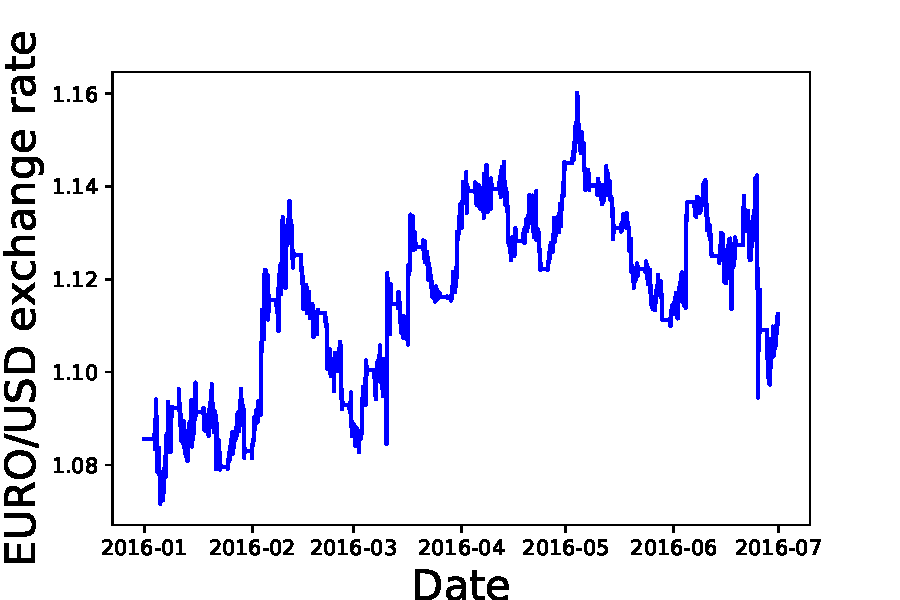
\includegraphics[scale=0.4]{EURO_USD_exchange_rate.pdf}
\caption{The exchange rate from EUR to USD from Jan 2016 to Jul 2016.}
\label{fig:EURUSD example}
\centering
\end{center}
\end{figure}


\subsection{Project Statement}
%In this section, you will want to clearly define the problem that you are trying to solve, including the strategy (outline of tasks) you will use to achieve the desired solution. You should also thoroughly discuss what the intended solution will be for this problem. Questions to ask yourself when writing this section:
%
%Is the problem statement clearly defined? Will the reader understand what you are expecting to solve?
%Have you thoroughly discussed how you will attempt to solve the problem?
%Is an anticipated solution clearly defined? Will the reader understand what results you are looking for?

The main objective of this project will be to use classical and more recent machine learning techiques to make forecasts of different time series with the goal of applying the best methods to predict currency exchange rates. The simplest model that we will use is the ARIMA model, defined in the previous section as the baseline model. The ARIMA model has been shown to be adequate in estimating the exchange rates of certain currencies Ref.~\cite{Mong_2016}. We will then use different neural networks architectures such as the feed forward and long-short term memory networks, as in Ref.~\cite{Chaudhuri_2016,Oancea_2014,Pant_2018}, to make predictions of time series and use our baseline models and root mean square differences to quantify and compare the performance of different forecasts.


\subsection{Metrics}
%In this section, you will need to clearly define the metrics or calculations you will use to measure performance of a model or result in your project. These calculations and metrics should be justified based on the characteristics of the problem and problem domain. Questions to ask yourself when writing this section:
%
%Are the metrics you’ve chosen to measure the performance of your models clearly discussed and defined?
%Have you provided reasonable justification for the metrics chosen based on the problem and solution?


There are several metrics that can be used to evaluate the predictions of our models Ref.~\cite{Adhikari_2013}, however, for our project we will focus on three commonly used metrics, the mean squared error, root mean squared error, and the Akaike information criterion. First we define some terminology, the forecast error, $e_t$, is
\begin{equation}
e_{t} = X_t - F_t,
\end{equation}
where $X_t$ is the value of the time series at time step $t$ and $F_t$ is the forecasted value at the same time step. The three metrics that we will use for our project are
\begin{enumerate}

\item  The mean square error (MSE)
\begin{itemize}
\item $\text{MSE} = \frac{1}{N}\sum\limits_{t=1}^{N} e^2_{t} $
\end{itemize}

\item  The root mean squared error (RMSE)
\begin{itemize}
\item $\text{RMSE} = \sqrt{\frac{1}{N}\sum\limits_{t=1}^{N} e^2_{t}} $
\end{itemize}

\item The Akaike information criterion (AIC)
\begin{itemize}
\item $\text{AIC} = 2k - \text{Ln}(\hat{L})$
\end{itemize}
where $k$ is the number of parameters in the model and $\hat{L}$ is the maximum value of the likelyhood function for the model.

\end{enumerate}
\noindent
The MSE and RMSE metrics were chosen because, unlike other metrics such as the mean-absolute error (MAE), the MSE and RMSE more strongly penalize the forecast error $e_t$ due to their quadratic dependence $e^2_t$. Therefore, large deviations of the forecast to the true data are strongly penalized. Because I was interested in forecasting models which strongly penalized outliers in the forecasts, the MSE and RMSE metrics were the most appropriate. The AIC metric was chosen for evaluating the ARIMA and SARIMA models because it is a well established method for ARIMA and SARIMA models. The AIC scores the specified model on the assumption that the true model of the underlying time series is of higher dimensions than what is being evaluated. Another metric that would be appropriate is the Bayesian information criterion (BIC). The Bayesian information criterion will penalize models more based on the number of present parameters. However, since the AIC has been shown to be asymptotically equivilent to cross-validation \cite{Stone_1977}, it will produce better fits than the BIC metric and was the reason that we chose it. In these three cases, the smaller that the value of the RMSE, MSE, and AIC is, then the better the overall model.

\newpage
\section{Analysis}
%(approx. 2-4 pages)

\subsection{Data Exploration}
%In this section, you will be expected to analyze the data you are using for the problem. This data can either be in the form of a dataset (or datasets), input data (or input files), or even an environment. The type of data should be thoroughly described and, if possible, have basic statistics and information presented (such as discussion of input features or defining characteristics about the input or environment). Any abnormalities or interesting qualities about the data that may need to be addressed have been identified (such as features that need to be transformed or the possibility of outliers). Questions to ask yourself when writing this section:
%
%If a dataset is present for this problem, have you thoroughly discussed certain features about the dataset? Has a data sample been provided to the reader?
%If a dataset is present for this problem, are statistics about the dataset calculated and reported? Have any relevant results from this calculation been discussed?
%If a dataset is not present for this problem, has discussion been made about the input space or input data for your problem?
%Are there any abnormalities or characteristics about the input space or dataset that need to be addressed? (categorical variables, missing values, outliers, etc.)
We focused on three time series data sets. {\bf i}.~The international airline passenger data set, containing the total number of airline passengers in thousands from Jan 1949 until Dec 1960; {\bf ii}.~The sunspot data set, showing the monthly number of sunspots from 1705-1989; {\bf iii}.~The EUR to USD exchange rate from Jan 2016- July 2016. Datasets {\bf i}.~ and {\bf ii}.~ both consist of two columns, one for the time steps $t$ and the values being measured $X_t$. 

\begin{table}[h]
\centering
\begin{tabular}{ c c }
Month $(t)$ & Int. airline passengers $(X_t)$ \\ \hline
 1949-01 & 112 \\ 
 1949-02 & 118  \\  
 1949-03 & 132   \\
 \vdots & \vdots 
\end{tabular}
\caption{The format of datasets {\bf i}.~and {\bf ii}.}
\label{table: sample format of dataset i and ii}
\end{table}

The third data set, {\bf iii}.~contains several columns related to the exchange rate market. The columns are Time, the Opening rate, the maximum value of the rate , the lowest value , the closing exchange rate value, and the total volume of the exchange market.

\begin{table}[h]
\centering
\begin{tabular}{ c c c c c c }
            Time &     Open &    High &    Low &   Close   &  Volume \\ \hline
2010-01-01 00:00 &  1.43283 & 1.43293 & 1.43224 & 1.43293 & 608600007.1 \\
2010-01-01 00:15 &  1.43285 & 1.43295 & 1.43229 & 1.43275 & 535600003.2 \\
2010-01-01 00:30 &  1.43280 & 1.43303 & 1.43239 & 1.43281 &  436299999.2 \\
\vdots  &  \vdots  & \vdots  & \vdots  & \vdots  &  \vdots 
\end{tabular}
\caption{A sample of the format of dataset {\bf iii}.}
\label{table: sample format of dataset iii}
\end{table}
To help us better understand our datasets, in Table \ref{table: descriptive statistics of datasets}, we give the computed descriptive statistics of our three data sets in comparison to one-another.

\begin{table}[h]
\centering
\begin{tabular}{c | c | c | c}
     &    Data set {\bf i.} & Data set {\bf ii.} &  Data set {\bf iii.} \\ \hline
count &  144 & 309 & 245441  \\
mean &  280.298611 & 49.752104 & 1.268375  \\
std  &  119.966317 & 40.452595 & 0.112992  \\
min  &  104.000000 & 0.0000000 & 1.035580 \\
25$\%$  &  180.000000 & 16.000000 & 1.135360 \\
50$\%$  &  265.500000 & 40.000000 & 1.302350  \\
75$\%$  &  360.500000 & 69.800000 & 1.356560 \\
max  &  622.000000 &  190.200000 & 1.493240 
\end{tabular}
\caption{Descriptive statistics of the data sets {\bf i}, {\bf ii}.~and {\bf iii}.}
\label{table: descriptive statistics of datasets}
\end{table}

\newpage
\subsection{Exploratory Visualization}
%In this section, you will need to provide some form of visualization that summarizes or extracts a relevant characteristic or feature about the data. The visualization should adequately support the data being used. Discuss why this visualization was chosen and how it is relevant. Questions to ask yourself when writing this section:
%
%Have you visualized a relevant characteristic or feature about the dataset or input data?
%Is the visualization thoroughly analyzed and discussed?
%If a plot is provided, are the axes, title, and datum clearly defined?
%
To understand the data in a more visual way, in the figures below, we plot the times series data sets that we will be analyzing.

\begin{figure}[h]
\centering
\begin{subfigure}{.5\textwidth}
  \centering
  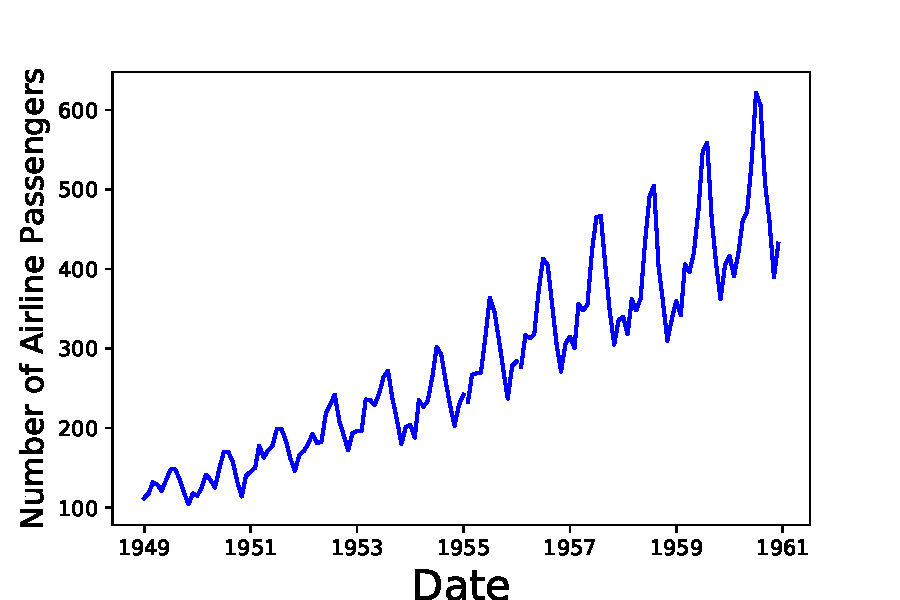
\includegraphics[scale=0.41]{Airline_Passengers.pdf}
  \caption{The number of airline passengers\\ from 1949-1961.}
  \label{fig:Airline example}
\end{subfigure}%
\begin{subfigure}{.5\textwidth}
  \centering
  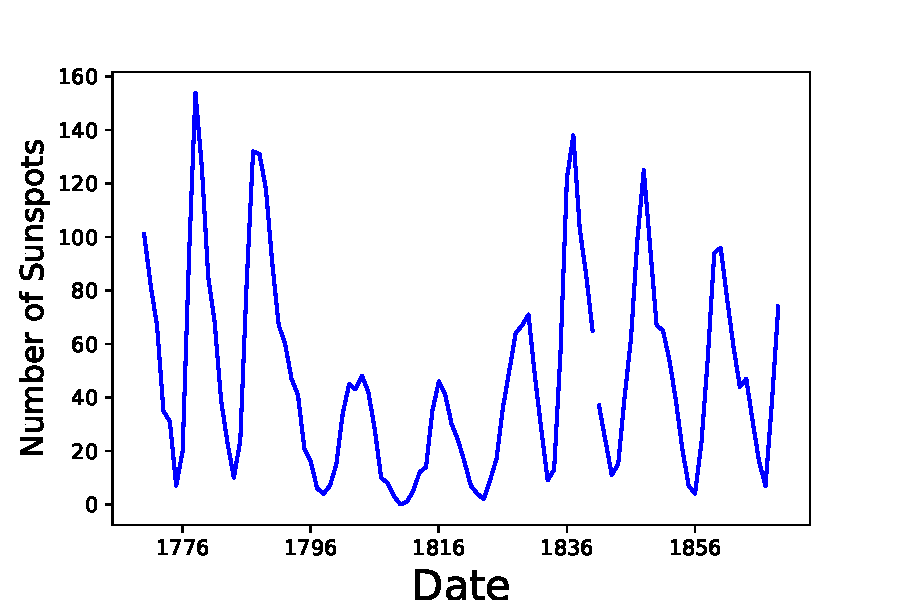
\includegraphics[scale=0.41]{Sunspot.pdf}
 \caption{The number of observed sunspots from 1705-1989. }
  \label{fig:Sunspot example}
\end{subfigure}
\caption{A figure with two subfigures}
\label{fig:test}
\end{figure}


The airline data set in Fig.~\ref{fig:Airline example} shows two interesting patterns, the general increasing number of airline passengers over time, along with a seasonal yearly pattern. The sunspot data set in Fig.~\ref{fig:Sunspot example} shows a cyclical pattern that repeats about every 11-years.

\begin{figure}[h]
\begin{center}
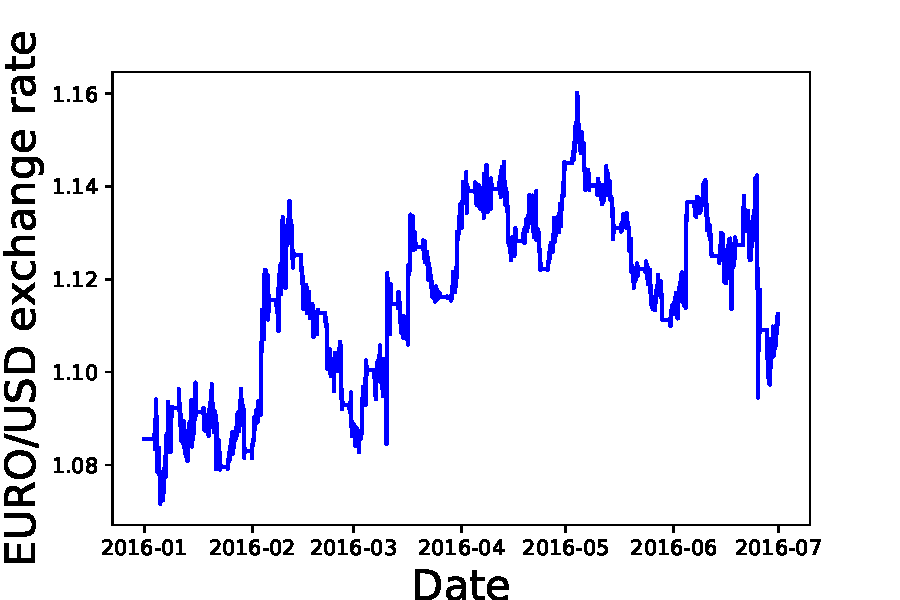
\includegraphics[scale=0.4]{EURO_USD_exchange_rate.pdf}
\caption{The exchange rate from EUR to USD from Jan 2016 to Jul 2016.}
\label{fig:EURUSD example2}
\centering
\end{center}
\end{figure}

In Fig.~\ref{fig:EURUSD example2} we plot the Euro to USD closing price from Jan 2016 to July 2016. There does not seem to be any apparent seasonal or cyclical patterns in this data sample.


\subsection{Algorithms and Techniques}
%In this section, you will need to discuss the algorithms and techniques you intend to use for solving the problem. You should justify the use of each one based on the characteristics of the problem and the problem domain. Questions to ask yourself when writing this section:
%
%Are the algorithms you will use, including any default variables/parameters in the project clearly defined?
%Are the techniques to be used thoroughly discussed and justified?
%Is it made clear how the input data or datasets will be handled by the algorithms and techniques chosen?
For this project, we will use the ARIMA model as a benchmark model as described in Sec.~\ref{sec: overview} and implemented as in Sec.~\ref{section: Fitting ARIMA}. ARIMA models have been used to predict foreign exchange rates \cite{Mong_2016} and are a classical method for time series forecasts Ref.~\cite{Adhikari_2013}. For these reasons, we use the ARIMA model as a benchmark.


Neural networks for time series models have been explored in the literature  \cite{Adhikari_2013,Oancea_2014,Chaudhuri_2016} and have shown good predictive abilities. This motivates us to explore neural networks for our forecasts. The two neural networks that we will use is the feed-forward neural network with a variable number of nodes along with a long-short-term memory network with a variable number of LSTM units. These networks are shown schematically in Figs.~\ref{fig:FFNN architecture} and \ref{fig:LSTM architecture} in the case of 4 nodes and 4 LSTM units. The tutorials in Refs.~\cite{Acatay_2017,Pant_2018,Vincent_2018} were very instructive in getting started with these models.
\begin{figure}[h]
\begin{center}
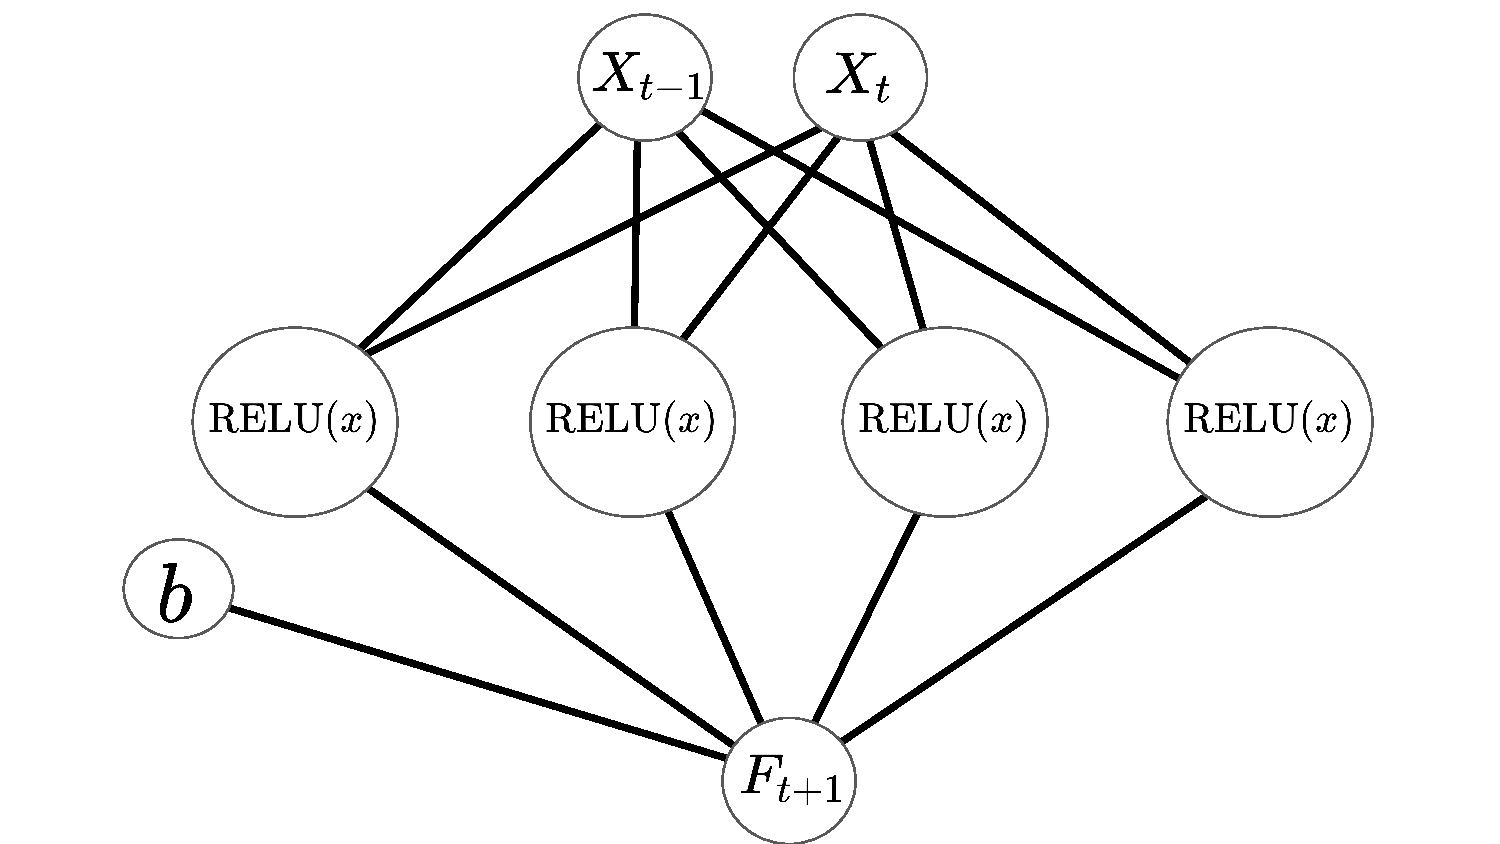
\includegraphics[scale=0.4]{Neural_net_schematic_FFNN.pdf}
\caption{The chosen feed-forward neural network architecture.}
\label{fig:FFNN architecture}
\centering
\end{center}
\end{figure}
In this diagram, ${X_{t-1},X_{t}}$ is the time series pair that is fed into the neural network, ${\rm RELU}(x)$ is the rectified linear unit activation function of the network, $b$ is the bias parameter, and $F_{t}$ is the forecast of the model.
\begin{figure}[h]
\begin{center}
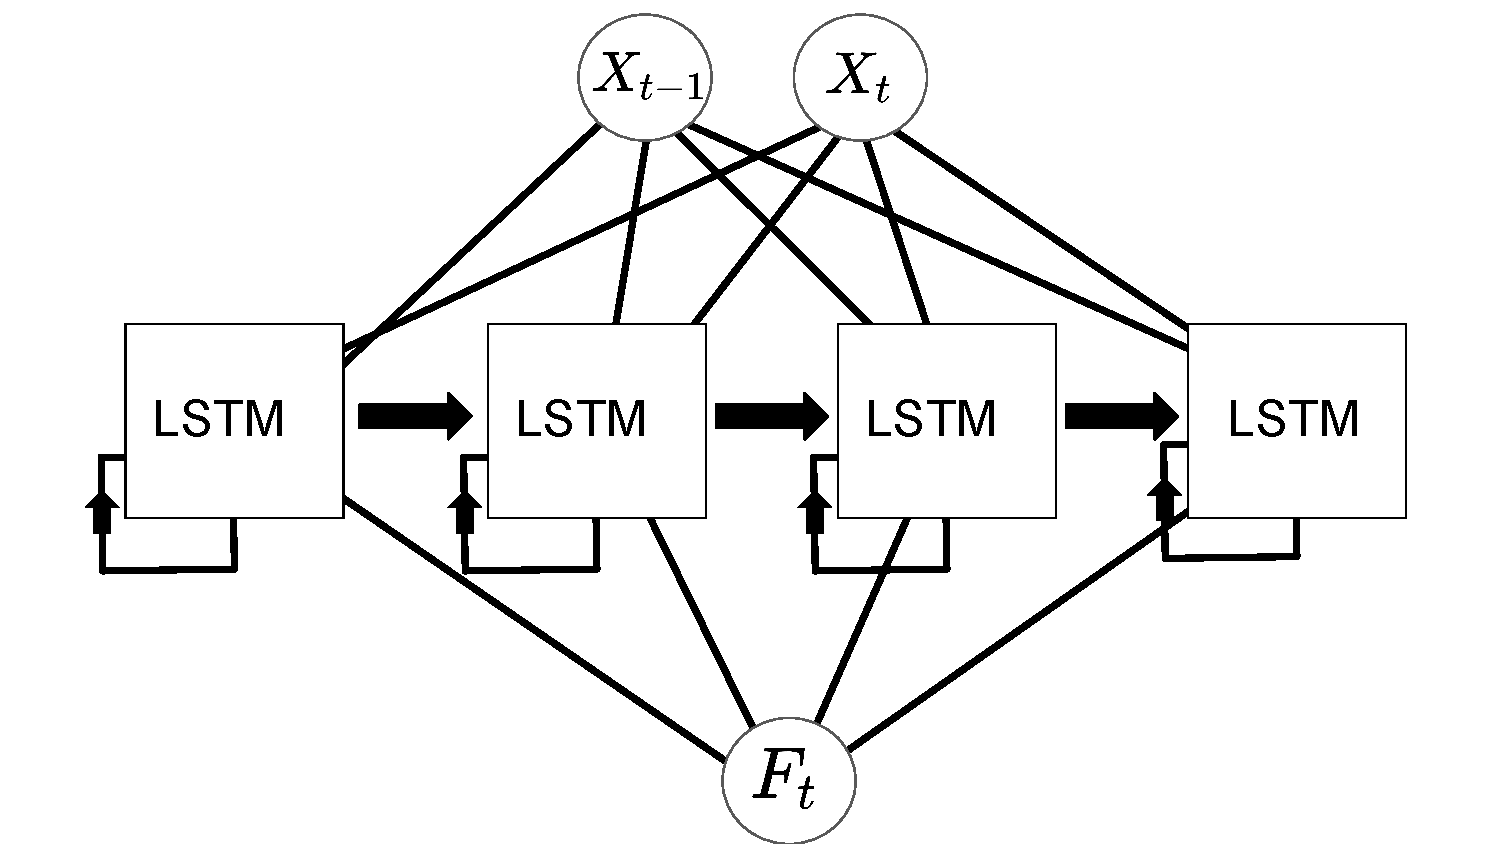
\includegraphics[scale=0.4]{Neural_net_schematic_LSTM.pdf}
\caption{The chosen LSTM neural network architecture.}
\label{fig:LSTM architecture}
\centering
\end{center}
\end{figure}
As in the previous diagram, ${X_{t-1},X_{t}}$ is the time series pair. The LSTM blocks represent the long-short-term memory units which feed out-put data back into themselves and $F_{t}$ is the prediction. In both of the cases, the final model is able to generate a prediction $F_{t+1}$ for the time series based on the value of the time series at the current time step $X_{t}$. In Sec.~\ref{section: Fitting NN}, we will discus how these architectures were implemented in python.


\subsection{Benchmark}

%In this section, you will need to provide a clearly defined benchmark result or threshold for comparing across performances obtained by your solution. The reasoning behind the benchmark (in the case where it is not an established result) should be discussed. Questions to ask yourself when writing this section:
%
%Has some result or value been provided that acts as a benchmark for measuring performance?
%Is it clear how this result or value was obtained (whether by data or by hypothesis)?
%

The ARIMA model and seasonal ARIMA model were fit with optimized grid-search parameters, as described in Sec.~\ref{section: Fitting ARIMA}, with optimized parameters given in Table \ref{table: optimal fitting parameters ARIMA}. In Fig.~\ref{fig:Airline ARIMA forecast}, Fig.~\ref{fig:Sunspot ARIMA forecast} and Fig.~\ref{fig:EURUSD ARIMA forecast} the curve in blue is the training data used for fitting, the green line in the testing data and the red lines and red shaded area show the average value of the ARIMA forecast with the 95$\%$ confidence regions of the predictions.
\begin{figure}[h]
\centering
\begin{subfigure}{.5\textwidth}
  \centering
  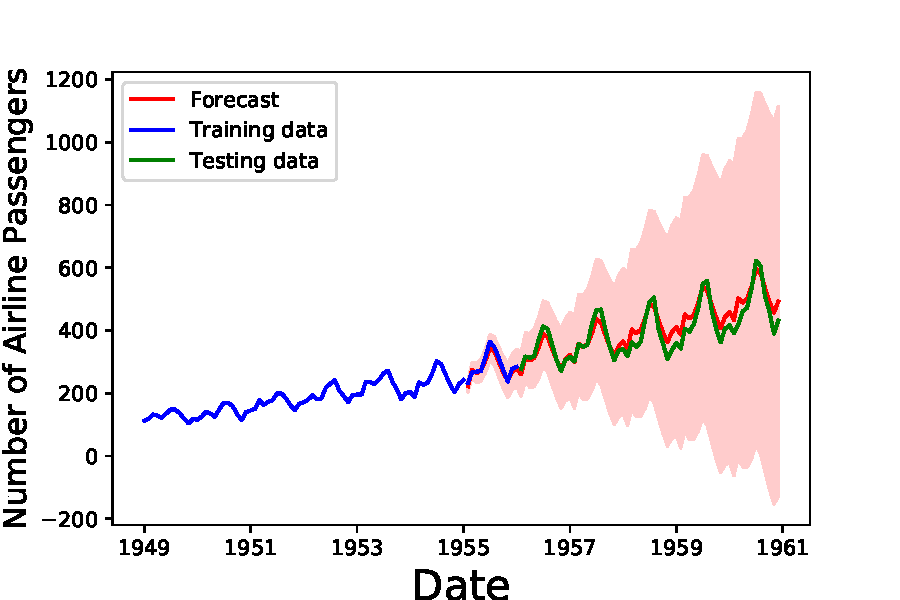
\includegraphics[scale=0.41]{Airline_Passengers_Forecast.pdf}
  \caption{SARIMA results}
  \label{fig:Airline ARIMA forecast}
\end{subfigure}%
\begin{subfigure}{.5\textwidth}
  \centering
  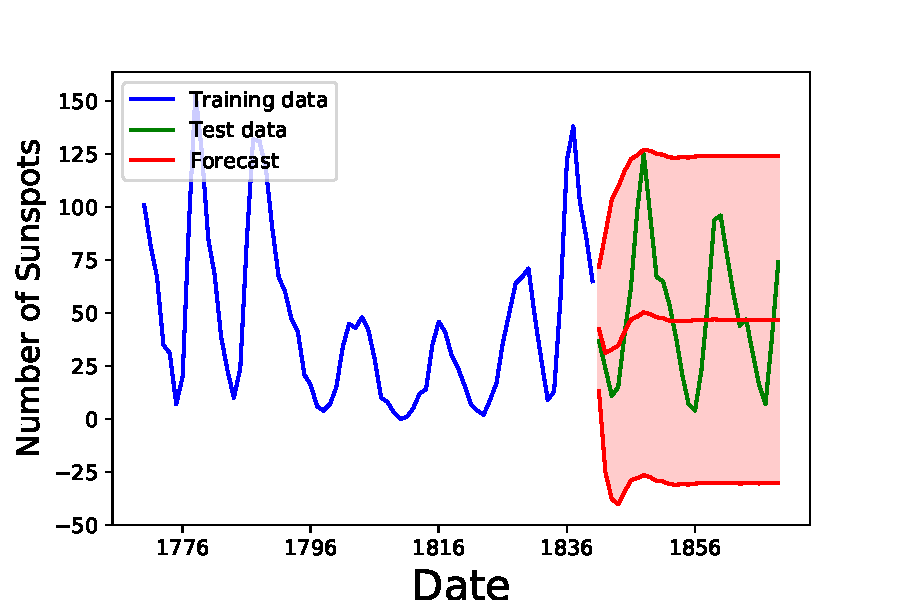
\includegraphics[scale=0.41]{Sunspot_Forecast.pdf}
\caption{ARIMA results}
  \label{fig:Sunspot ARIMA forecast}
\end{subfigure}
\caption{A figure with two subfigures}
\label{fig: Airline and SUNSPOT ARIMA}
\end{figure}
In Fig.~\ref{fig:Airline ARIMA forecast}, we see that the SARIMA model was able to correctly find the overall trend and as time increases, the forecast uncertainty also increases as would be expected. Fig.~\ref{fig:Sunspot ARIMA forecast} which used a ARIMA model, did not seem to to detect the correct trend and produces an uncertainty band that does not change over time. However, the height of the band does overlap with the training data. 

\begin{figure}[h]
\begin{center}
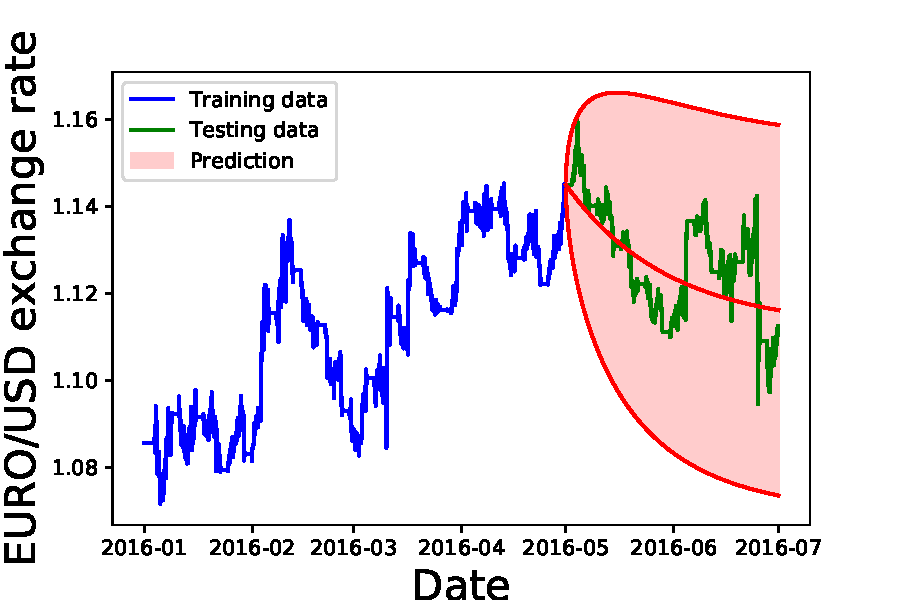
\includegraphics[scale=0.4]{EURO_USD_exchange_rate_with_Forecast.pdf}
\caption{The forecasted exchange rate from EUR to USD from Jan 2016 to Jul 2016.}
\label{fig:EURUSD ARIMA forecast}
\centering
\end{center}
\end{figure}

In Fig.~\ref{fig:EURUSD ARIMA forecast} above, we see that the ARIMA model did not do a very good job at reproducing the data and it predicts a decreasing trend over time. The uncertainty band is very large in this case and encompasses a wide scale. In Table \ref{table: RMS values of benchmark models}, we provide the MSE and RMSE values of the optimized ARIMA and SARIMA models for the above data sets.

\begin{table}[h]
\centering
\begin{tabular}{lccc}
Data Set & Model & MSE & RMSE \\ \hline
{\bf i.} & SARIMA & 1878.63101438 & 43.3431772529 \\
{\bf ii.} & ARIMA & 902.466806466 & 30.0410853077 \\
{\bf iii.} & ARIMA & 8.67079188384e-05  &  0.00931170869596 \\ \hline
\end{tabular}
\caption{The RMS and RMSE values of the benchmark models.}
\label{table: RMS values of benchmark models}
\end{table}

%
\section{Methodology}
%(approx. 3-5 pages)
%
\subsection{Data Preprocessing}
%In this section, all of your preprocessing steps will need to be clearly documented, if any were necessary. From the previous section, any of the abnormalities or characteristics that you identified about the dataset will be addressed and corrected here. Questions to ask yourself when writing this section:
%
%If the algorithms chosen require preprocessing steps like feature selection or feature transformations, have they been properly documented?
%Based on the Data Exploration section, if there were abnormalities or characteristics that needed to be addressed, have they been properly corrected?
%If no preprocessing is needed, has it been made clear why?
%Implementation
%In this section, the process for which metrics, algorithms, and techniques that you implemented for the given data will need to be clearly documented. It should be abundantly clear how the implementation was carried out, and discussion should be made regarding any complications that occurred during this process. Questions to ask yourself when writing this section:
%
%Is it made clear how the algorithms and techniques were implemented with the given datasets or input data?
%Were there any complications with the original metrics or techniques that required changing prior to acquiring a solution?
%Was there any part of the coding process (e.g., writing complicated functions) that should be documented?
%Refinement
%In this section, you will need to discuss the process of improvement you made upon the algorithms and techniques you used in your implementation. For example, adjusting parameters for certain models to acquire improved solutions would fall under the refinement category. Your initial and final solutions should be reported, as well as any significant intermediate results as necessary. Questions to ask yourself when writing this section:
%
%Has an initial solution been found and clearly reported?
%Is the process of improvement clearly documented, such as what techniques were used?
%Are intermediate and final solutions clearly reported as the process is improved?

The forecasting models that we used in this work only require the values ($t,X_t$), since the data sets that we used do not contain any missing values, our data sets did not require any cleanup. However, it was necessary to scale the data, from $X_t \rightarrow \tilde{X}_t$ for the neural network data so that it was in the range $[0,1]$. This transformation was accomplished using the following scaling function
\begin{equation}
 \tilde{X}_t = \frac{ X_t - X_{\rm min}}{X_{\rm max} - X_{\rm min}},
\end{equation} 
where $X_{\rm max}, X_{\rm min}$ are the maximal and minimum values of the data sets, respectively. This is implemented in python as the following code snippet.
\begin{lstlisting}
def scale_array(y_vec):
    
    ymax = np.max(y_vec)
    ymin = np.min(y_vec)
    
    y_vec_scaled = np.zeros((len(y_vec),1))
    
    for k in range(0,len(y_vec)):
        y_vec_scaled[k][0] = (y_vec[k][0]-ymin)/(ymax-ymin)
    
    return y_vec_scaled,ymin,ymax
\end{lstlisting}

To invert the value from the scaling function, we use,
\begin{equation}
X_{t} = X_{\rm min} + \tilde{X}_t\cdot \left(X_{\rm max} - X_{\rm min} \right).
\end{equation}
The inversion of the transformation was carried out after the model made its predictions so that the predictions would be in the original range of the data set. This is implemented as follows,
\begin{lstlisting}
def invert_scaling(y_vec_scaled,ymin,ymax):
    
    y_vec = np.zeros(y_vec_scaled.shape)
        
    for k in range(0,len(y_vec_scaled)):
        y_vec[k] = ymin+(ymax-ymin)*y_vec_scaled[k]
    return y_vec
\end{lstlisting}
In order to train the neural network models, we used the following arrays as our feature matrix $X$ and the training data $y$
\begin{align}
X_{\rm Train} &= [{X_{1},X_2,X_3, ..., X_T}], \\
y_{\rm Train} &= [{X_{2},X_3,X_4, ..., X_{T+1}}].
\end{align}
In order to generate these two arrays we used the following function
\begin{lstlisting}
def future_data(data,lags=1,future=1):
    '''
    This function, takes in the time series [X_t] and returns the array
    X=[X_{t}]
    Y=[X_{t+1}]
    '''
    
    X, y = [], []
    for row in range(len(data) - lags - future):
        a = data[row:(row + lags), 0]
        X.append(a)
        y.append(data[row + lags+future-1, 0])
    return np.array(X), np.array(y)
\end{lstlisting}
Another data prepossessing step that we carried out was to separate out the data into training vs testing data sets. The usual amount of training vs testing was about 60-80$\%$ for training and 30-40$\%$ testing.

There were some additional complications that arose during the coding phases. These complications were related to the some formatting issues that I was not used to.
\begin{itemize}
\item The \verb|statsmodel| package expected the dataframe containing the \verb|pandas| data frame to
have a specific time-format. It took me some time to learn that when I read in data into the dataframe, I needed to use the \verb|dataframe.strftime("%Y-%m")| to set the column correctly.
\item It was difficult to find the correct batch size number for fitting the model, when I used a large number, the resulting models seemed to do very poorly which was counter-intuitive. Smaller batch sizes seemed to give better results.
\item The more parameters I was optimizing with the grid search, the longer the runtime. This was a problem with the LSTM network where it was particularly slow.
\end{itemize}



\subsection{ARIMA Model: Implementation}\label{section: Fitting ARIMA}

We used the ARIMA and the Seasonal ARIMA models from the python package \verb|statsmodels| (Ref.~\cite{Skipper_2010}). The ARIMA model consists of the variables $(p,d,q)$, which are the non-seasonal AR order, differencing, and MA order, respectively. In order to fit this model to data, we use grid search from $(p,d,q)=(0,0,0) \rightarrow (p_{\rm Max},d_{\rm Max},q_{\rm Max}) $. To fit the ARIMA model we chose to either minimize the AIC, or the root mean square (RMS) value. The following code generates the grid that we will use to search the model space for the best fitting ARIMA model,
\begin{lstlisting}
	p = range(0,pMax+1)
	d = range(0,dMax+1)
	q = range(0,qMax+1)
	
	# This creates all combinations of p,q,d
	pdq = list(itertools.product(p, d, q))
\end{lstlisting}
For each item in the grid generated with the previous code snippet, we fit ARIMA$(p,d,q)$ model using the following code.
\begin{lstlisting}
for param in pdq:
		arma_mod = statsmodels.tsa.arima_model.ARIMA(train_data,order=param).fit()
\end{lstlisting}
Once the model is fit, the AIC or RMS value is computed and the set of parameters $(p,d,q)$ that generated the best score is taken to be the optimal model.\\


The seasonal ARIMA model incorporates non-seasonal and seasonal factors as a multiplicative model. Therefore, we can schematically write
\begin{equation}
{\rm SARIMA} = {\rm ARIMA}(p,d,q) \times {\rm S}(P,D,Q,T),
\end{equation}
where the variables $(p,d,q)$ are the non-seasonal AR order, differencing, and MA order, respectively. The variables $(P,D,Q)$ denote the same variables, except for the seasonal component $S$. The variable $T$ denotes the number of time steps for a single period. For example, if the time units are in months, then $T$=6 indicates a half-year seasonal pattern. In order to fit the SARIMA$(p,q,d,P,D,Q,T)$ model to data, we use a gridsearch. The following code snippet generates a grid of $(p,d,q)=(0,0,0) \rightarrow (p_{\rm Max},d_{\rm Max},q_{\rm Max}) $ and $(P,D,Q)=(0,0,0) \rightarrow (p_{\rm Max},d_{\rm Max},q_{\rm Max},T) $, where we take $T$ as fixed, for simplicity.
\begin{lstlisting}
	p = range(0,pMax+1)
	d = range(0,dMax+1)
	q = range(0,qMax+1)
	t = [t]
	
	# This creates all combinations of p,q,d
	pdq = list(itertools.product(p, d, q))
	
	# This creates all combinations of the seasonal variables
	seasonal_pdq = [(x[0], x[1], x[2], x[3]) for x in list(itertools.product(p, d, q,t))]
\end{lstlisting}
For each combination, $(p,q,d,P,D,Q,T)$, we fit the SARIMA model using the code below.
\begin{lstlisting}
	for param in pdq:
		for param_seasonal in seasonal_pdq:
					mod = sm.tsa.statespace.SARIMAX(train_data,
                            					    order=param,
                            	  seasonal_order=param_seasonal,
                                     enforce_stationarity=False,
                                    enforce_invertibility=False)
				   results = mod.fit()
\end{lstlisting}


Using the above prescription for fitting the ARIMA and SARIMA models, the following table summarizes the results of the gridsearch.
\begin{table}[h]
\centering
\begin{tabular}{l | c | c | c}
 Data Set    &    Model  & Optimal $(p,d,q)$ &  Optimal $(P,S,Q,T)$ \\ \hline
{\bf i.} Airline Passengers & SARIMA & $(1, 1, 1)$ & $(1, 0, 0, 12)$ \\
{\bf ii.} Sunspots & ARIMA  & $(5,0,4)$ & - \\
{\bf iii.} EUR to USD rate & ARIMA & (2, 0, 2) & - 
\end{tabular}
\caption{The optimal fitting parameters of the ARIMA, or SARIMA model.}
\label{table: optimal fitting parameters ARIMA}
\end{table}


\subsection{Neural Network Model: Implementation}\label{section: Fitting NN}
The feed-forward neural network in Fig.~\ref{fig:FFNN architecture} is implemented in Keras. In order to find the optimal number of nodes in this model, we performed a cross-validated grid-search of the parameters \verb|neurons| (the number of nodes to use in the network) and the \verb|batch_size| (the number of training samples used in one iteration during training). The cross validation was performed using the following code snippet, which constructs the model in the function \verb|build_model(neurons)|
and then finds the best fit using the \verb|GridSearchCV| function.
\begin{lstlisting}
from sklearn.model_selection import GridSearchCV
from keras.wrappers.scikit_learn import KerasRegressor

def build_model(neurons):
   '''
   This function build the Feed Forward Neural Network model with a variable number of nodes.
   '''
    model = Sequential()
    model.add(Dense(neurons, input_dim=lags, activation=activation_func))
    model.add(Dense(1))
    model.compile(loss='mean_squared_error', optimizer='adam')
    return model

# Construct the Regressor model
regressor = KerasRegressor(build_fn = build_model,verbose=0)
parameters = {'batch_size': [5,10,20], # Take half of the training data
              'epochs': [number_of_epochs],
              'neurons': [4,5,10,15,20]}
              
grid_search = GridSearchCV(estimator = regressor,
                           param_grid = parameters,
                           scoring = 'neg_mean_squared_error',
                           cv = 10)
                           
# Fit the various models using the object defined above
grid_search = grid_search.fit(X_train, y_train)
best_parameters = grid_search.best_params_
best_accuracy = grid_search.best_score_
\end{lstlisting}

Once the optimal parameters have been found, we construct this model with the following code snippet that also using the \verb|mean_squared_error| metric and the \verb|adam| optimizer.
\begin{lstlisting}
# Now we build and train the optimal model
model = build_model(neurons=best_parameters['neurons'])

# Store the history of loss of the optimal function
history=model.fit(X_train, y_train, epochs=best_parameters['epochs'], batch_size=best_parameters['batch_size'], verbose=0)
\end{lstlisting}
The following is an example summary of this implemented architecture (when the optimal nodes is four)
\begin{lstlisting}
Layer (type)                 Output Shape              Param #   
=================================================================
dense_1 (Dense)              (None, 4)                 8         
_________________________________________________________________
dense_2 (Dense)              (None, 1)                 5         
=================================================================
Total params: 13
Trainable params: 13
Non-trainable params: 0
_________________________________________________________________
\end{lstlisting}
Using the same optimizer, loss function and the \verb|GridSearchCV| object as the feed-forward neural network the LSTM network is implemented as follows
\begin{lstlisting}
def build_model(neurons):
    model = Sequential()
    model.add(Dense(neurons, input_dim=lags, activation=activation_func))
    model.add(Dense(1))
    model.compile(loss='mean_squared_error', optimizer='adam')
    return model
\end{lstlisting}
Below, we give and example of the LSTM network summary of an implemented LSTM network in the case that the optimal model had four LSTM units,
\begin{lstlisting}
Layer (type)                 Output Shape              Param #   
=================================================================
lstm_1 (LSTM)                (None, 4)                 96        
_________________________________________________________________
dense_1 (Dense)              (None, 1)                 5         
=================================================================
Total params: 101
Trainable params: 101
Non-trainable params: 0
_________________________________________________________________
\end{lstlisting}


\section{Results}
%(approx. 2-3 pages)
%
\subsection{Model Evaluation and Validation}
%In this section, the final model and any supporting qualities should be evaluated in detail. It should be clear how the final model was derived and why this model was chosen. In addition, some type of analysis should be used to validate the robustness of this model and its solution, such as manipulating the input data or environment to see how the model’s solution is affected (this is called sensitivity analysis). Questions to ask yourself when writing this section:
%
%Is the final model reasonable and aligning with solution expectations? Are the final parameters of the model appropriate?
%Has the final model been tested with various inputs to evaluate whether the model generalizes well to unseen data?
%Is the model robust enough for the problem? Do small perturbations (changes) in training data or the input space greatly affect the results?
%Can results found from the model be trusted?
Having implemented the feed forward and LSTM networks in Keras as described in Sec.~\ref{section: Fitting NN} we fit the model and generate the time series predictions $\lbrace F_t \rbrace$. One issue that we had using this model was that the predictions of the neural networks do not produce any uncertainties. To try to probe the uncertainties of the model, we carried out the following procedure \\
\begin{enumerate}
\item Train the model using the set $\lbrace X_{T,{\rm Train}} \rbrace$
\item Using the training data, calculate the predictions $\lbrace F_{T,{\rm Train}} \rbrace$
\item Compute the mean squared error (RMSE), and the standard deviation $\sigma_{\rm RMS}$ between the training set $X_{T,{\rm Train}}$ and the prediction on the training set $F_T$.
\item We generate the perturbation, $\delta X_{T}$, assumed to be a Gaussian random variable sampled from the distribution $ \mathcal{N}(\frac{1}{2}{\rm RMS},\frac{1}{2}\sigma_{\rm RMS} )$
\item We added the perturbation to the test data $X_T +\delta X_{T}$ and generate predictions on the testing set, $\lbrace F_{T,{\rm Test}} \rbrace$.
\item We repeat this process many times, until we generate a distribution of forecasts. The distribution of the forecasts will be the estimated uncertainty of the neural network predictions.
\end{enumerate}
Using this procedure, we generated the uncertainty bands in Figs.~\ref{fig:results Airline},\ref{fig:results sunspots},\ref{fig:results EURO_USD}.
\begin{figure}[h]
\centering
\begin{subfigure}{.5\textwidth}
  \centering
  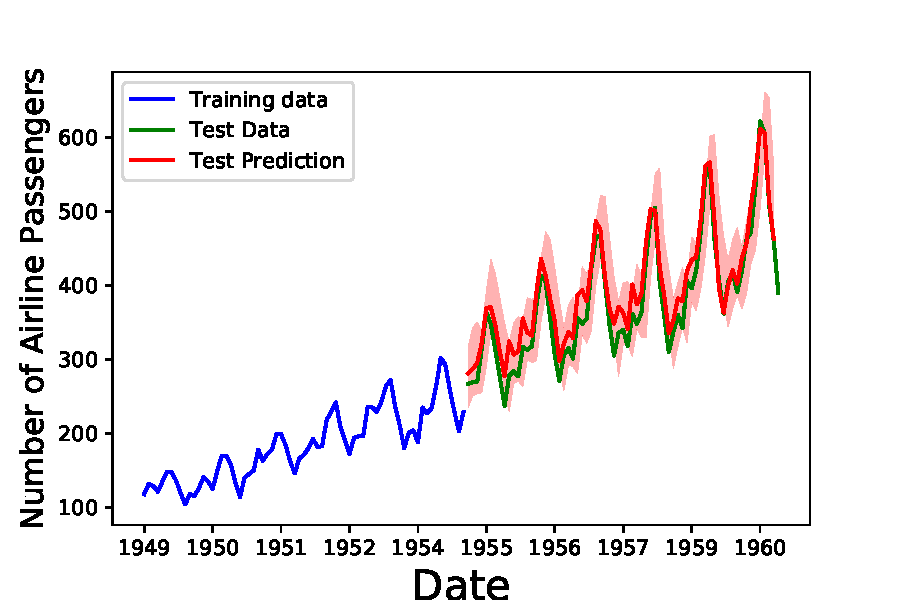
\includegraphics[scale=0.41]{Airline_Passengers_NN.pdf}
  \caption{FFNN results}
  \label{fig:NN results Airline}
\end{subfigure}%
\begin{subfigure}{.5\textwidth}
  \centering
  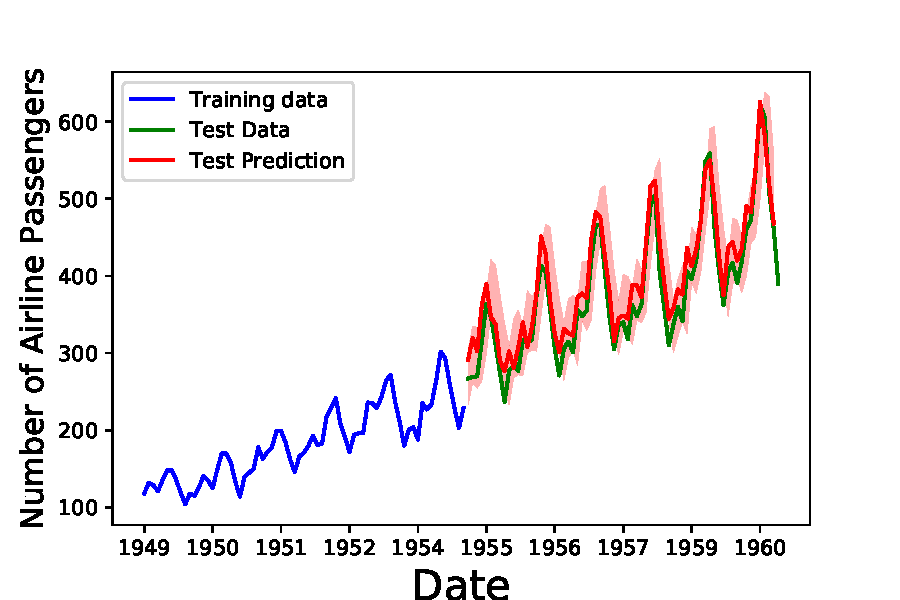
\includegraphics[scale=0.41]{Airline_Passengers_LSTN.pdf}
  \caption{LSTM results}
  \label{fig:LSTM results Airline}
\end{subfigure}
\caption{(a) The predictions with uncertainty of the feed forward neural network model. (b) The predictions with uncertainty of the LSTM model. }
\label{fig:results Airline}
\end{figure}
In Fig.~\ref{fig:results Airline} we plot the predictions of the feed forward and LSTM neural networks for the Airline passengers dataset. In both cases the red uncertainty band overlap the actual training data, indicating a good fit.

\begin{figure}[h]
\centering
\begin{subfigure}{.5\textwidth}
  \centering
  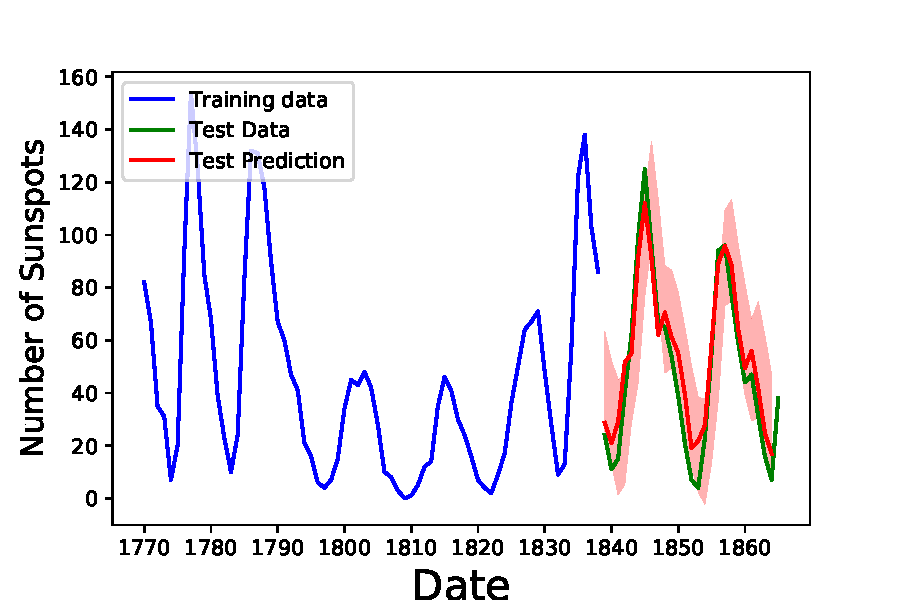
\includegraphics[scale=0.41]{Sunspot_Forecast_NN.pdf}
  \caption{FFNN results}
  \label{fig:NN results sunspots}
\end{subfigure}%
\begin{subfigure}{.5\textwidth}
  \centering
  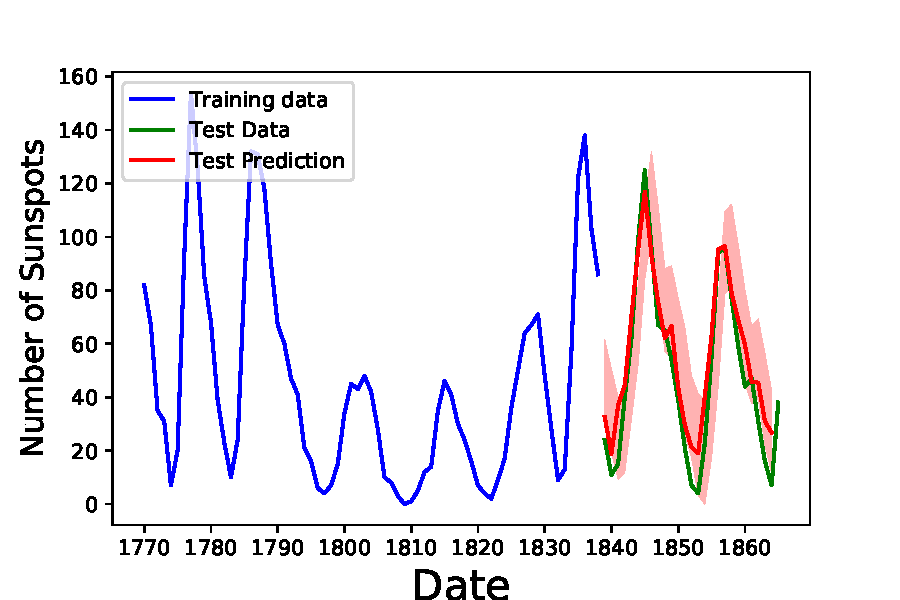
\includegraphics[scale=0.41]{Sunspot_Forecast_LSTN.pdf}
  \caption{LSTM results}
  \label{fig:LSTM results sunspots}
\end{subfigure}
\caption{(a) The predictions with uncertainty of the feed forward neural network model. (b) The predictions with uncertainty of the LSTM model.}
\label{fig:results sunspots}
\end{figure}
In Fig.~\ref{fig:results sunspots} we show the comparison of the FFNN and LSTM results for the sunspot dataset. In this case we also see that the uncertainty bands are in agreement with the training data.

\newpage
\begin{figure}[h]
\centering
\begin{subfigure}{.5\textwidth}
  \centering
  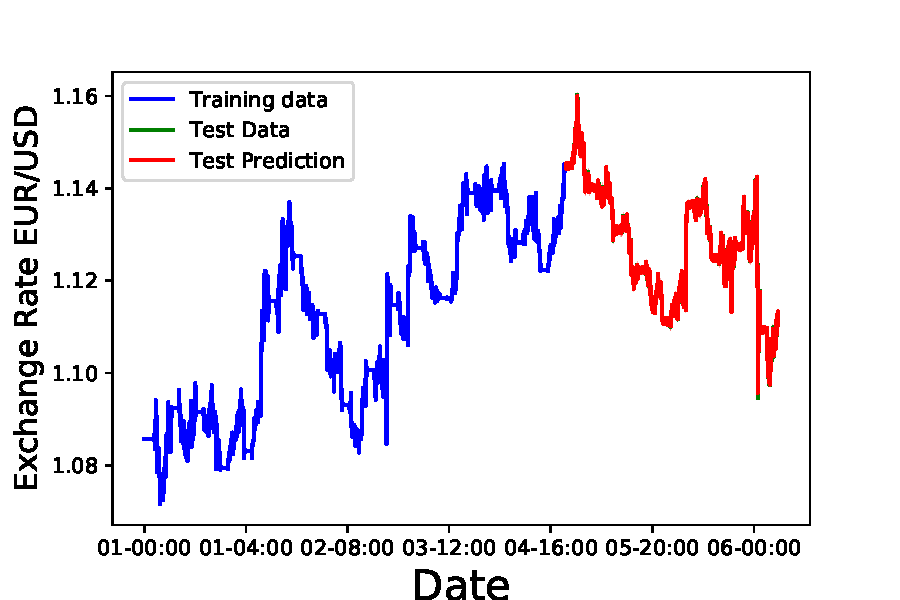
\includegraphics[scale=0.41]{EURO_USD_exchange_rate_NN.pdf}
  \caption{FFNN results}
  \label{fig:NN results EURO_USD}
\end{subfigure}%
\begin{subfigure}{.5\textwidth}
  \centering
  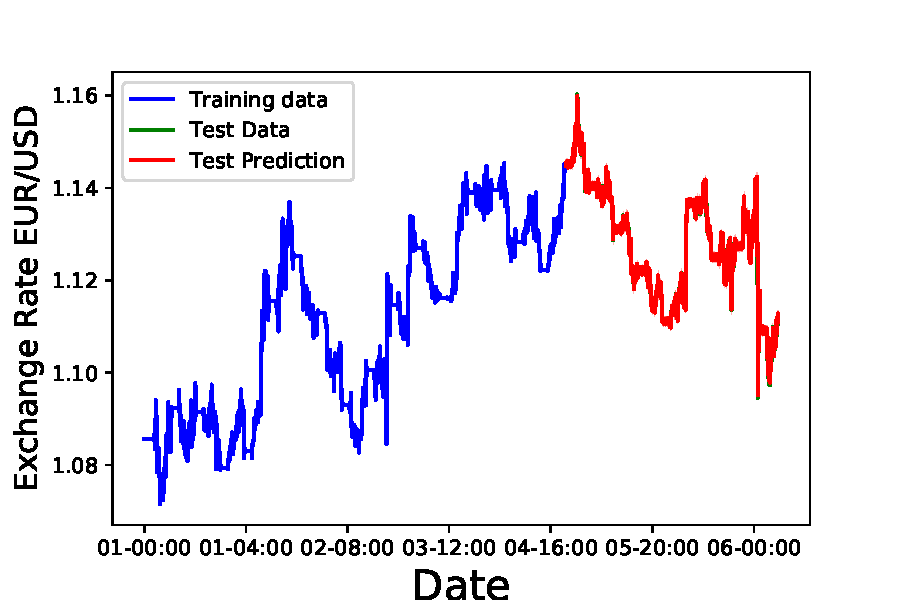
\includegraphics[scale=0.41]{EURO_USD_exchange_rate_LSTN.pdf}
  \caption{LSTM results}
  \label{fig:LSTM results EURO_USD}
\end{subfigure}
\caption{(a) The predictions with uncertainty of the feed forward neural network model. (b) The predictions with uncertainty of the LSTM model.}
\label{fig:results EURO_USD}
\end{figure}
In Fig.~\ref{fig:results EURO_USD} we show the results of the FFNN and LSTM networks on the Euro to USD exchange rate. In this case the estimated uncertainty was very small, therefore the uncertainty bands are not visible in the scale of the figure.


\subsection{Justification}
%In this section, your model’s final solution and its results should be compared to the benchmark you established earlier in the project using some type of statistical analysis. You should also justify whether these results and the solution are significant enough to have solved the problem posed in the project. Questions to ask yourself when writing this section:
%
%Are the final results found stronger than the benchmark result reported earlier?
%Have you thoroughly analyzed and discussed the final solution?
%Is the final solution significant enough to have solved the problem?
In Table \ref{table: RMS values of neural network models}, we give the final MSE and RMSE values of all models considered in this project. The RMSE baseline ratio is the value of the RMSE of the baseline model over the RMSE value of the specific model. The larger this ratio, the better the selected model is compared to the baseline model.
\begin{table}[h]
\centering
\begin{tabular}{cccc|c}
Data Set & Model & MSE & RMSE  & RMSE Baseline Ratio\\ \hline
{\bf i.} & SARIMA & 1878.638 & 43.343 & 1 \\
{\bf i.} & FFNN & 604.999 & 24.597 &  1.76 \\
{\bf i.} & LSTM & 567.813 & 23.829 &  1.82 \\ \hline 
{\bf ii.} & ARIMA & 902.467 & 30.041 & 1 \\
{\bf ii.} & FFNN & 101.171 & 10.058 &  2.99\\
{\bf ii.} & LSTM & 119.393 & 10.927 &  2.75 \\ \hline
{\bf iii.} & ARIMA & 8.671 $\times 10^{-5}$  &  9.312 $\times 10^{-3}$ & 1 \\
{\bf iii.} & FFNN & 7.243 $\times 10^{-8}$ & 2.691 $\times 10^{-4}$ &  34.6 \\
{\bf iii.} & LSTM & 8.454 $\times 10^{-8}$ & 2.908 $\times 10^{-4}$ &  32.0 \\ \hline
\end{tabular}
\caption{The RMS and RMSE values of the Feed Forward (FFNN) and long-short term memory (LSTM) neural network model results.}
\label{table: RMS values of neural network models}
\end{table}
In all three cases, we have that the FFNN and LSTM models outperformed the baseline SARIMA and ARIMA models\footnote{ We note that the values in this table will vary slightly in every run by up to 10$\%$ for the MSE and about 3$\%$ for the RMSE. However, the order of magnitude of these values remain the same.}. The FFNN and LSTM models for data sets {\bf i.} outperformed the baseline by a factor of 1.8, while in data set {\bf ii.} they outperformed the baseline roughly by a factor of 3. For dataset {\bf iii.}, the FFNN and LSTM models  outperformed the baseline by a factor of about 30. We also observed that in some data sets, the LSTM models outperformed the FFNN models by a small margin, however as a rigorous statistical analysis of the RMS and RMSE metrics were not carried out in this project, this small difference is probably not statistically significant. 
\newpage
\section{Conclusion}
%(approx. 1-2 pages)
%
\subsection{Free-Form Visualization}
%In this section, you will need to provide some form of visualization that emphasizes an important quality about the project. It is much more free-form, but should reasonably support a significant result or characteristic about the problem that you want to discuss. Questions to ask yourself when writing this section:
%
%Have you visualized a relevant or important quality about the problem, dataset, input data, or results?
%Is the visualization thoroughly analyzed and discussed?
%If a plot is provided, are the axes, title, and datum clearly defined?
While we had a good amount of success in making models for the time series we considered, it is important to note that not all time series can be tackled using the neural network architectures in this project. There were cases where good fits did not seem to be possible, like the ``Annual rainfall in London (in inches)'' data set shown in the figure below. When I first looked at this data set, I tried to fit it using the methods that I described in this project, but I obtained very poor results, as pictured in Fig.~\ref{fig:results FNN rainfall}. I tried increasing the training set, changing the activation functions, adding more nodes, but it did not fix the quality of the prediction. It would be very interesting in the future to investigate why this type of time series did not produce good results.
\begin{figure}[h]
\centering
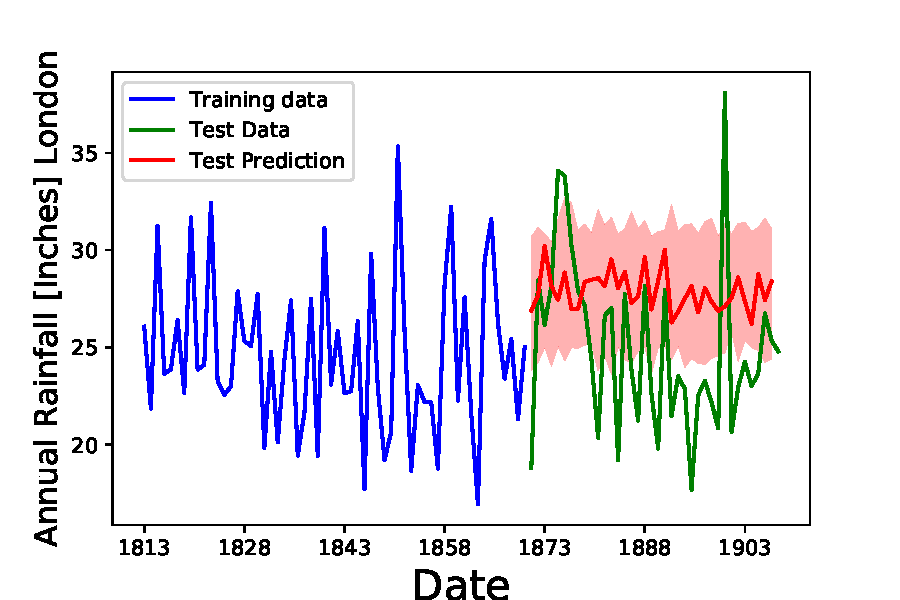
\includegraphics[scale=0.41]{Annual_Rainfall_NN_relu.pdf}
\caption{The predictions with uncertainty of the FFNN model with a RELU activation function.}
\label{fig:results FNN rainfall}
\end{figure}




\subsection{Reflection}
%In this section, you will summarize the entire end-to-end problem solution and discuss one or two particular aspects of the project you found interesting or difficult. You are expected to reflect on the project as a whole to show that you have a firm understanding of the entire process employed in your work. Questions to ask yourself when writing this section:
%
%Have you thoroughly summarized the entire process you used for this project?
%Were there any interesting aspects of the project?
%Were there any difficult aspects of the project?
%Does the final model and solution fit your expectations for the problem, and should it be used in a general setting to solve these types of problems?
In this project we have taken data for time series data $(t,X_t)$ and we have trained two different neural network models, the feed forward neural network (FFNN) and the Long-short term memory (LSTM) network, denoted as $G_{\rm FFNN}$ ,$G_{\rm LSTM}$ respectively; to generate a time series forecast given the value of the time series at the previous time step. In other words, we have generated a function $G$ such that
\begin{equation}
G(X_{t}) = F_{t+1}
\end{equation}
where $F_{t+1}$ should be similar to the $X_{t+1}$ value of the underlying time series data. This problem was very interesting to me as it introduced me to how complicated and difficult time-series analysis can be, the body of literature that studies this subject is large, so it was great to be able to learn a little about it. The project had some challenges, mainly in getting started and in trying to understand the different approaches to time series modeling. The final model worked better than I expected and it is worth investigating in a more rigorous fashion. The fact that the FFNN and LSTM models outperformed the baseline by such a large margin for the EUR/USD exchange rate data suggests that perhaps the model was over-fitting. In the future, I would like to carry out more stringent tests to check against the over-fitting hypothesis.
 

\subsection{Improvements}
%In this section, you will need to provide discussion as to how one aspect of the implementation you designed could be improved. As an example, consider ways your implementation can be made more general, and what would need to be modified. You do not need to make this improvement, but the potential solutions resulting from these changes are considered and compared/contrasted to your current solution. Questions to ask yourself when writing this section:
%
%Are there further improvements that could be made on the algorithms or techniques you used in this project?
%Were there algorithms or techniques you researched that you did not know how to implement, but would consider using if you knew how?
%If you used your final solution as the new benchmark, do you think an even better solution exists?

There are some further improvements that we could have carried out to the implemented models, such as an in-depth exploration of different neural network topologies. Adding more adding more layers would have been interesting to explore. However I ran out of time before I could carry out such a careful study. In the future I would also like to implement a generative adversarial artificial neural network for time series prediction. There was not enough time to understand and implement this model, but it seemed quite interesting and powerful. I will try to extend my project in the future to do this.


%Before submitting, ask yourself. . .
%
%Does the project report you’ve written follow a well-organized structure similar to that of the project template?
%Is each section (particularly Analysis and Methodology) written in a clear, concise and specific fashion? Are there any ambiguous terms or phrases that need clarification?
%Would the intended audience of your project be able to understand your analysis, methods, and results?
%Have you properly proof-read your project report to assure there are minimal grammatical and spelling mistakes?
%Are all the resources used for this project correctly cited and referenced?
%Is the code that implements your solution easily readable and properly commented?
%Does the code execute without error and produce results similar to those reported?




\newpage
\begin{thebibliography}{9}

\bibitem{Adhikari_2013}
R. Adhikari and R. K. Agrawal, An Introductory Study on Time Series Modeling and Forecasting, 2013, [arXiv:1302.6613] \url{https://arxiv.org/abs/1302.6613}.

\bibitem{Mong_2016}
T. Mong and U. Ngan, Research Journal of Finance and Accounting www.iiste.org
ISSN 2222-1697 (Paper) ISSN 2222-2847 (Online)
Vol.7, No.12, 2016 \url{http://iiste.org/Journals/index.php/RJFA/article/viewFile/31511/32351}.

\bibitem{Patel_2014} P. J. Patel,  N. J. Patel and A. R. Patel, IJAIEM 3, 3, 2014. \url{http://www.ijaiem.org/volume3issue3/IJAIEM-2014-03-05-013.pdf}

% Neural networks for time Series
\bibitem{Oancea_2014} B. Oancea, S. Cristian Ciucu, Proceedings of the CKS 2013, [arXiv:1401.1333] \url{https://arxiv.org/abs/1401.1333}.

% Neural network time series  
\bibitem{Chaudhuri_2016} T. D. Chaudhuri and I. Ghosh,	Journal of Insurance and Financial Management, Vol. 1, Issue 5, PP. 92-123, 2016,  [arXiv:1607.02093] \url{https://arxiv.org/abs/1607.02093}.

% Tutorial for LSTM for time series 
\bibitem{Pant_2018} Pant, N. (2017, September 07). A Guide For Time Series Prediction Using Recurrent Neural Networks (LSTMs). Retrieved from \url{https://blog.statsbot.co/time-series-prediction-using-recurrent-neural-networks-lstms-807fa6ca7f}.


% Tutorial for Feed forward neural network
\bibitem{Acatay_2017} D. K. Acatay, (2017, Nov. 21) Part 6: Time Series Prediction with Neural Networks in Python. Retrieved from \url{http://dacatay.com/data-science/part-6-time-series-prediction-neural-networks-python/}

\bibitem{Vincent_2018} Vincent, T. (2018). ARIMA Time Series Data Forecasting and Visualization in Python | DigitalOcean. [online] digitalocean.com. Available at: \url{https://www.digitalocean.com/community/tutorials/a-guide-to-time-series-forecasting-with-arima-in-python-3} [Accessed 29 Jul. 2018].

\bibitem{Esteban_2017} C. Esteban, S. L. Hyland and G R\"{a}tsch, \url{https://github.com/ratschlab/RGAN} [arXiv:1706.02633]. 

\bibitem{Skipper_2010} S. Skipper and J. Perktold. ``Statsmodels: Econometric and statistical modeling with python." Proceedings of the 9th Python in Science Conference. 2010. \url{https://www.statsmodels.org/stable/index.html}

\bibitem{Stone_1977} Stone, M. ``An Asymptotic Equivalence of Choice of Model by Cross-Validation and Akaike's Criterion.” Journal of the Royal Statistical Society. Series B (Methodological), vol. 39, no. 1, 1977, pp. 44–47. JSTOR, JSTOR, \url{www.jstor.org/stable/2984877}.



\end{thebibliography}
\end{document}